\section{Recursos principals del bloc persones}

    \paragraph{}
    El centre d'aquest bloc de recursos és el recurs Persona. Aquest recurs, emmagatzema els detalls que identifiquen i caracteritzen a cada una de les persones de l'arbre així com la informació bàsica sobre els seus relatius més propers.

    D'aquest recurs principal, pengen els enllaços cap als recursos que permeten obtenir informació sobre els relatius de la persona, els estudis realitzats sobre aquesta, l'historial de canvis, les fonts d'informació i les memòries afegides pels usuaris.

    La imatge [ref] ofereix una visió de l'esquema que acabem de descriure i permet veure com el recurs Persona s'enllaça amb la resta de blocs que conformen l'arbre familiar~\ref{img:personsBloc}.

    \begin{figure}[h]
        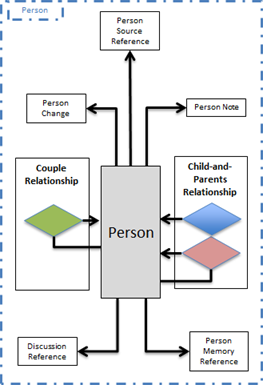
\includegraphics{05/03_personsCore}
        \centering
        \caption{El bloc de l'arbre familiar relatiu a les Persones.}\label{img:personsBloc}
    \end{figure}

    Aquest bloc de recursos és el més gran de tots i pràcticament, emmagatzema tota la informació rellevant dels individus accessibles a través de l'API. En els següents subapartats s'exposaran els diferents recursos que conformen aquest bloc i quines són les peces d'informació utilitzables que aquests contenen.

    Podreu observar, en les taules que representen l'estructura dels recursos, que a vegades, per la columna que marca el format de dades d'un paràmetre, aquest es troba especificat entre els caràcters `[' i `]'. Aquesta terminologia s'utilitza per indicar que aquest paràmetre és en realitat un recurs o objecte de dades diferent inclòs dins del recurs estudiat.

    També s'observarà que sovint, els recursos exposats, hereten dades d'altres recursos i en els casos que aquests siguin rellevants, se n'exposarà l'estructura a l'apartat `Altres recursos interessants', més endavant en la memòria.

    \subsection{El recurs Persona (Person)}

    \paragraph{}
    El recurs Persona és el primer objecte amb què cal familiaritzar-se per tal de comprendre la potencialitat emmascarada d'aquesta API.

    Cada instància, fa referència a una persona diferent de l'arbre familiar i generalment, representa el punt d'entrada per tal d'accedir a tota la informació disponible sobre un individu, ja sigui perquè aquesta es troba inclosa en el recurs o esdevé accessible a través dels enllaços hypermedia.

    Els enllaços hypermedia del recurs Persona permeten accedir a la informació relativa als seus avantpassats, descendents, artefactes, historial de canvis, parelles, discussions, notes i fonts de dades.

    Les dades pròpies pel recurs Persona poden ser observades a la taula~\ref{tab:person}. Cal recordar que aquest recurs també hereta els paràmetres dels recursos Subjecte, Conclusió, Enllaços Hypermedia i Dades Extensibles que poden ser trobats a la secció `Altres recursos interessants'.

    \begin{center}
             \csvreader[
                separator=comma,
                before table=\sffamily\small,
                longtable={p{2cm-2\tabcolsep}p{3.5cm-2\tabcolsep}p{8.5cm-2\tabcolsep}},
                table head={\caption{Codificació GEDCOM X del recurs Persona}\label{tab:person}\\\toprule%
                    \headentry{m{2cm-2\tabcolsep}}{Paràmetre}
                    & \headentry{m{3.4cm-2\tabcolsep}}{Format de Dades}
                    & \headentry{m{8.5cm-2\tabcolsep}}{Descripció}\\\midrule},
                late after line=\\\midrule,
                late after last line=\\\bottomrule,
             ]
             {./tables/05/01_persons/person.csv}
             {param=\param,format=\format,desc=\desc}
             {\param&\format&\desc}
     \end{center}

    \subsection{El recurs Gènere (Gender)}

    \paragraph{}
    El recurs Gènere s'utilitza per especificar el gènere d'una persona en concret. Aquest recurs conté els paràmetres propis mostrats a la taula~\ref{tab:gender} i hereta els camps de dades dels recursos , Conclusió, Enllaços Hypermedia i Dades Extensibles que poden ser trobats a la secció `Altres recursos interessants'.

    \begin{center}
             \csvreader[
                separator=comma,
                before table=\sffamily\small,
                longtable={p{2cm-2\tabcolsep}p{3.5cm-2\tabcolsep}p{8.5cm-2\tabcolsep}},
                table head={\caption{Codificació GEDCOM X del recurs Persona}\label{tab:gender}\\\toprule%
                    \headentry{m{2cm-2\tabcolsep}}{Paràmetre}
                    & \headentry{m{3.4cm-2\tabcolsep}}{Format de Dades}
                    & \headentry{m{8.5cm-2\tabcolsep}}{Descripció}\\\midrule},
                late after line=\\\midrule,
                late after last line=\\\bottomrule,
             ]
             {./tables/05/01_persons/gender.csv}
             {param=\param,format=\format,desc=\desc}
             {\param&\format&\desc}
     \end{center}


     \subsubsection{L'enumeració genderType}

     \paragraph{}
     L'enumeració genderType segueix l'estructura de definició GEDCOMX. Com a tal, els valors possibles per l'enumeració segueixen la pauta:\\\verb|http://gedcomx.org/ + `genderType'|

     La següent taula mostra els tres possibles valors de l'enumeració genderType.

     \begin{center}
         \csvreader[
            no head,
            separator=comma,
            table head={\caption{Valors possibles per genderType}\label{tab:genderType}},
            before table=\sffamily\small,
            longtable={|p{3cm}|p{3cm}|p{3cm}|},
            column count=4,
            late after head=\\\hline,
            late after line=\\\hline,
            late after last line=\\\hline,
         ]
         {./tables/05/01_persons/genderType.csv}
         {1=\one,2=\two,3=\three}
         {\one&\two&\three}
     \end{center}

